\chapter{AI-Driven Design with Ollama}

\section{Prompt Engineering}
Provide the AI with context: current endpoints, latency goals, blocked regions, and risk appetite. Keep prompts short; ask for structured bullet plans.

\section{Closed-Loop Automation}
\begin{figure}[h]
    \centering
    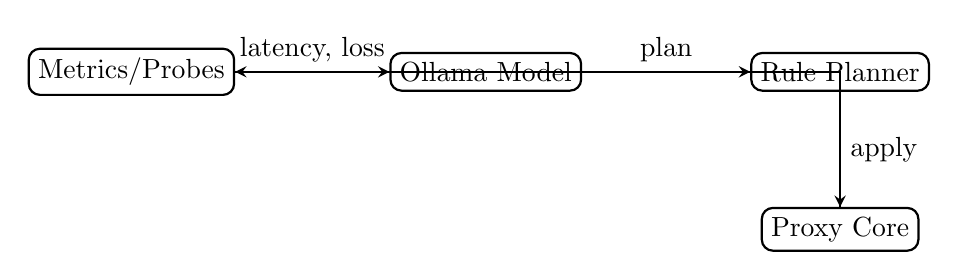
\begin{tikzpicture}[node distance=2cm,>=stealth,thick]
        \node (metrics) [draw, rounded corners] {Metrics/Probes};
        \node (ai) [draw, rounded corners, right of=metrics, xshift=2.5cm] {Ollama Model};
        \node (planner) [draw, rounded corners, right of=ai, xshift=2.5cm] {Rule Planner};
        \node (core) [draw, rounded corners, below of=planner] {Proxy Core};
        \draw[->] (metrics) -- node[above]{latency, loss} (ai);
        \draw[->] (ai) -- node[above]{plan} (planner);
        \draw[->] (planner) -- node[right]{apply} (core);
        \draw[->] (core) |- (metrics);
    \end{tikzpicture}
    \caption{Feedback loop keeps routes healthy and policies updated.}
\end{figure}

\section{Safety Rails}
\begin{itemize}
    \item Validate AI outputs before applying (schema + sandbox).
    \item Rate-limit reconfiguration to avoid flapping.
    \item Keep human-in-the-loop for sensitive regions.
\end{itemize}

\section{Prompt Patterns That Work Well}
\begin{itemize}
    \item \textbf{Structured bullets}: ask for ``Endpoints:``, ``Rules:``, ``Risks:`` sections.
    \item \textbf{Constraints}: explicitly set MTU, cipher preferences, and budget for endpoints.
    \item \textbf{Diff mode}: pass previous plan and ask only for changes to reduce noise.
\end{itemize}

\section{Schema Validation}
Wrap AI responses in JSON with a simple schema (endpoint list, rule list, rationale). Reject responses that fail validation and surface a clear error to the user.

\section{Practical Ollama Setup}
\begin{itemize}
    \item Run Ollama locally or remotely; set \texttt{OLLAMA\_HOST} and \texttt{OLLAMA\_MODEL}.
    \item Prefer smaller models for on-device proposals; larger ones for batch planning.
    \item Cache reusable suggestions (e.g., rule templates) to cut latency.
\end{itemize}

